\chapter{Prerequisiti}
%%%%%%%%%%%%%%%%%%%%%%%%%%%%%%%%%%%%%%%%%%%%55
%%%%%%%%%%%%%%%%%%%%%%%%%%%%%%%%5
%----------------------------------------------------------------------------------------
%	SECTION 
%----------------------------------------------------------------------------------------
\section{Funzione Obiettivo/Costo}
   In ottimizzazione matematica e nella teoria della decisione, una funzione \textbf{obiettivo} \cite{funzioneObiettivo} o di \textbf{costo} (detta anche loss function in inglese) è una funzione che mappa un evento, o valori di una o più variabili, su un numero reale intuitivamente rappresenta un "costo" associato all'evento. Un problema di ottimizzazione cerca di minimizzare una funzione di costo. In altri contesti, si può avere a che fare con una funzione obiettivo o la sua negata che deve essere massimizzata; si parla allora di funzione di rinforzo, funzione di utilità, funzione di fitness, ecc... . Viene in genere usata per stimare dei parametri ed è una funzione della differenza tra i valori attesi e quelli reali, per un'istanza di dati.
   \subsection{Selezione di una funzione obiettivo}
   Una buona pratica statistica richiede la selezione di una funzione di stima coerente con l'effettiva variazione sperimentata nel contesto di una particolare applicazione. Pertanto, nella pratica, la selezione del metodo statistico da utilizzare per modellare un problema applicato dipende dalla conoscenza dei costi che si verificheranno a causa delle circostanze specifiche al problema.
Un esempio comune riguarda la stima della "posizione". Sotto ipotesi statistiche tipiche, la media è il valore statistico usato per stimare quella posizione che minimizza l'errore con una funzione obiettivo quadratica, mentre la mediana è lo stimatore che minimizza l'errore con la funzione obiettivo che calcola la differenza assoluta. Stimatori si usano in altre circostanza, meno comuni. 
   Nell'apprendimento automatico, la funzione obiettivo è centrale nel processo di apprendimento poiché rappresenta la misura di quanto il sistema (tipicamente una rete neurale) apprende. Di conseguenza, la scelta della funzione obiettivo è strettamente legata alle prestazioni degli algoritmi perché questi sono orientati a ottenere i migliori valori possibili per la funzione, modificando, di conseguenza, i parametri del sistema (es: i pesi della rete) per avvicinarvisi. 
   \textbf{Due funzioni obiettivo molto comunemente usate sono l'errore quadratico medio.}
   \subsection{Nozioni aggiuntive}
   L'accuratezza dei una ipotesi si può misurare mediante una funzione di costo. Essa prende in input la differenza media di \textbf{tutte} i risultati $y$ che l'ipotesi fornisce in relazione a ogni esempio $x$ di un dataset.

\[J(\theta_0, \theta_1) = \dfrac {1}{2m} \displaystyle \sum _{i=1}^m \left ( \hat{y}_{i}- y_{i} \right)^2 = \dfrac {1}{2m} \displaystyle \sum _{i=1}^m \left (h_\theta (x_{i}) - y_{i} \right)^2\]
Tale funzione è chiamata \textbf{Funzione obiettivo quadratica} (\textit{Squared error function} oppure \textit{Mean squared error}). L'obiettivo principale è quello di rendere minima tale funzione di costo, al variare dei propri input. 
\begin{figure}[h!]
    \centering
    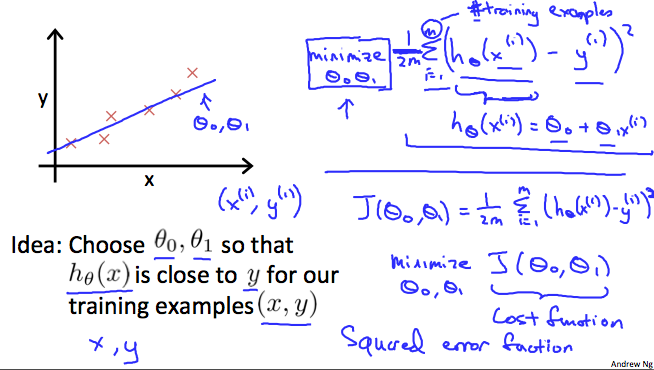
\includegraphics[width=1\textwidth]{img/R2YF5Lj3EeajLxLfjQiSjg_110c901f58043f995a35b31431935290_Screen-Shot-2016-12-02-at-5.23.31-PM.png}
\end{figure}
\begin{nota}
Non bisogna confondere la \textbf{funzione di costo/obiettivo} con l'ipotesi $h$ da attuare per \textit{"descrivere"} un insieme di dati:
\begin{itemize}
    \item $h_\theta(x)$ è una funzione di $x$ dato uno o più \textbf{valore fissati} $\theta_i$
    \item $J(\theta_1, \dots, \theta_n)$ è una funzione con parametri $\theta_1, \dots, \theta_n$.
\end{itemize}
\end{nota}
\begin{nota}
La funzione di costo \textbf{non} per forza deve essere una funzione quadratica, ne esistono molte altre. L'uso di una funzione obiettivo quadratica è comune (viene detta anche Loss L2), ad esempio quando si usano le tecniche dei minimi quadrati. Spesso una funzione quadratica è più matematicamente trattabile per via delle proprietà sulle varianze, oltre a essere simmetrica. 
Molti metodi statistici, tra cui il test t, l'analisi di regressione, la progettazione di esperimenti, eccetera, utilizzano il metodo dei minimi quadrati applicati usando la teoria della regressione lineare, che si basa su una funzione obiettivo quadratica. 
\end{nota}
\begin{esempio}
  Immaginiamo di porre $\theta_0 = 0$ per semplificare la funzione di costo: $J(\theta_0, \theta_1) = \dfrac {1}{2m} \displaystyle \sum _{i=1}^m \left ( \hat{y}_{i}- y_{i} \right)^2 = \dfrac {1}{2m} \displaystyle \sum _{i=1}^m \left (h_\theta (x_{i}) - y_{i} \right)^2$. \\ Il nostro obiettivo è quello di ottenere la miglior retta possibile che \textit{"approssima"} un determinato set di dati (\textit{regressione lineare}). In questo caso tale retta è simboleggiata dalla nostra ipotesi $h_\theta(x) = \theta_0 + \theta_1 x$. Nel prossimo paragrafo spiegheremo nel dettaglio come fare a ottenerla, per ora limitiamoci a pensare che bisogna far sì che $J(\theta_1) = 0$.\\
  Si prenda in considerazione il dataset seguente:\\
% Please add the following required packages to your document preamble:
% \usepackage[table,xcdraw]{xcolor}
% If you use beamer only pass "xcolor=table" option, i.e. \documentclass[xcolor=table]{beamer}
\begin{table}[H]
\centering
\begin{tabular}{|l|l|}
\hline
{\color[HTML]{FE0000} \textit{x}} & {\color[HTML]{FE0000} \textit{y(x)}} \\ \hline
1                                 & 1                                    \\ \hline
2                                 & 2                                    \\ \hline
3                                 & 3                                    \\ \hline
\end{tabular}
\end{table}
  Cominciamo a comporre la nostra funzione di costo per costruzione andando a variare i valori di $\theta_1$:\\
  Se $\theta_1 = 1$ allora  $h_\theta(x) = 0 + 1x = y(x) \,\,\,\,\,\,\forall x$. Di seguito evitiamo i calcoli e inseriamo una tabella con alcune approssimazioni:
  
% Please add the following required packages to your document preamble:
% \usepackage[table,xcdraw]{xcolor}
% If you use beamer only pass "xcolor=table" option, i.e. \documentclass[xcolor=table]{beamer}
\begin{table}[H]
\centering
\begin{tabular}{|l|l|}
\hline
{\color[HTML]{FE0000} \textit{$\theta_1$}} & {\color[HTML]{FE0000} \textit{$J(\theta_1)$}} \\ \hline
1                                          & 0                                    \\ \hline
0.5                                        & 0.58                                 \\ \hline
0                                          & 14/6                                 \\ \hline
\end{tabular}
\end{table}
Allora la funzione di costo $J$ sarà:
\begin{figure}[h!]
    \centering
    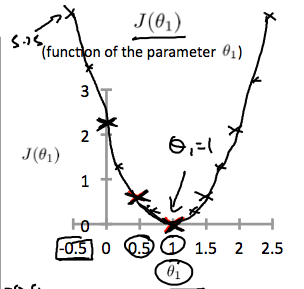
\includegraphics[width=0.7\textwidth]{img/fph0S5tTEeajtg5TyD0vYA_9b28bdfeb34b2d4914d0b64903735cf1_Screenshot-2016-10-26-01.09.05.png}
\end{figure}
\end{esempio}
\section{Discesa del gradiente}
Immaginiamo di avere una generica funzione $J(\theta_0 \dots \theta_n)$ per cui ne vogliamo trovare il valore minimo:
\[\min_{\theta_0 \dots \theta_n} J(\theta_0 \dots \theta_n)\]
Per farlo seguiamo i seguenti passaggi ipotetici:
\begin{itemize}
    \item Iniziamo con valori arbitrari di $\theta_i$
    \item Cambiamo tali valori finché non si arriva al minimo possibile.
\end{itemize}
Immaginiamo di basare la nostra funzione su due parametri ($\theta_0$ e $\theta_1$) e descriviamo il tutto mediante un grafico:
\begin{figure}[h!]
    \centering
    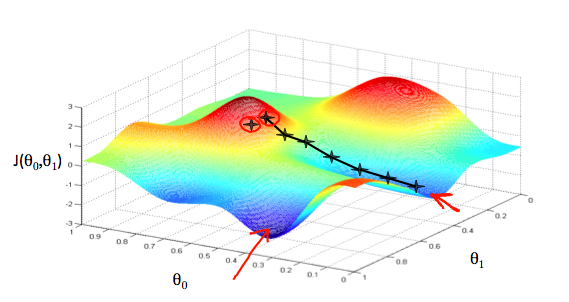
\includegraphics[width=1\textwidth]{img/bn9SyaDIEeav5QpTGIv-Pg_0d06dca3d225f3de8b5a4a7e92254153_Screenshot-2016-11-01-23.48.26.png}
    \caption{}\label{GradientDescent1}
\end{figure}
La figura \ref{GradientDescent1} mostra i punti risultati dal valore della funzione di costo nei punti $\theta_0$ e $\theta_1$. Le frecce rosse indicano alcuni dei possibili punti di minimo sul grafo. Il modo per fare ciò è quello di usare la \textbf{derivata} (la linea tangente alla funzione) della nostra funzione di costo. La pendenza (\textit{slope}) della tangente è la derivata in un punto e ci indica la direzione su cui "muoverci". In termini spiccioli: \textit{Scendiamo per la funzione di costo nella direzione con la discesa più ripida}. La \textbf{lunghezza} di ogni passo è determinato da un parametro, che precedentemente abbiamo chiamato \textbf{learning rate} $\alpha$. \\ Nella figura \ref{GradientDescent1} ogni "star" rappresentata sul grafo indica uno step determinato dal parametro $\alpha$. 
\begin{definizione}
    Un valore di $\alpha$ più piccolo darà vita a un passo in discesa più piccolo. Viceversa per valori più grandi.
\end{definizione}
\begin{definizione}
Dato un determinato valore di $\theta_0$ e $\theta_1$ (vale anche per i valori arbitrari dati a priori), la direzione da intraprendere è determinata dalla derivata parziale di della funzione di costo:
\[ \frac{\partial}{\partial \theta_j} J(\theta_0, \theta_1)\]
\end{definizione})  
L'algoritmo per la \textbf{discesa del gradiente} è il seguente:
\begin{algorithm}[H]
\begin{algorithmic}
        \While{La funzione non converge}
    \For{j = 0 to j = 1}
    \State{$\theta_j := \theta_j - \alpha \frac{\partial}{\partial \theta_j} J(\theta_0, \theta_1)$}
    \EndFor
    \EndWhile
    \end{algorithmic}
\end{algorithm}
Dove j indica gli indici delle features. A ogni iterazione $j$ i parametri $\theta_j$ vengono aggiornati \textbf{simultaneamente}.\\
Immaginiamo ora di avere, per semplicità, un solo parametro $\theta_1 \in \mathbb{R}$ da gestire:
\[\theta_1:=\theta_1-\alpha \frac{d}{d\theta_1} J(\theta_1)\]
Analizziamo una situazione fondamentale: il valore della derivata $\frac{d}{d\theta_1} J(\theta_1)$. Qualora essa sia \textbf{positiva} allora $\theta_1$ è destinato a \textbf{diminuire}, e viceversa (fig \ref{GradientDescent2}).
\begin{figure}[h!]
    \centering
    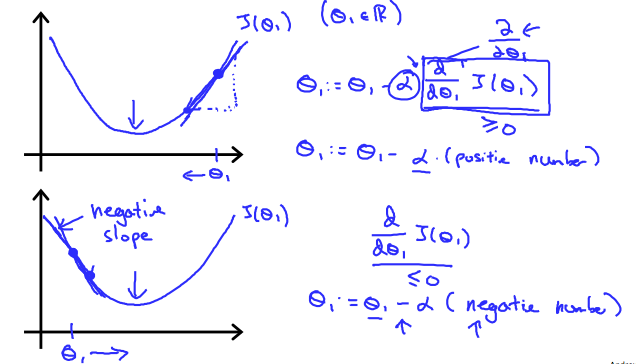
\includegraphics[width=1\textwidth]{img/SMSIxKGUEeav5QpTGIv-Pg_ad3404010579ac16068105cfdc8e950a_Screenshot-2016-11-03-00.05.06.png}
    \caption{}\label{GradientDescent2}
\end{figure}
\subsection{Descent Time}
A questo punto abbiamo intuito il perché molti denominano l'algoritmo come "\textit{Discesa del gradiente}", ma ci rimane da capire \textbf{quanto tempo} implica tale discesa.
In generale le tempistiche sono date da due fattori fondamentali:
\begin{itemize}
    \item Il valore di $\alpha$.
    \item Il valore della derivata.
\end{itemize}
Il primo aspetto da analizzare è la modifica del valore di $\alpha$ per garantire che il gradiente converga in un tempo accettabile. Un fallimento nella convergenza o una tempistica troppo elevata sono elementi caratterizzanti di un \textbf{learning rate} sbagliato.
\begin{figure}[h!]
    \centering
    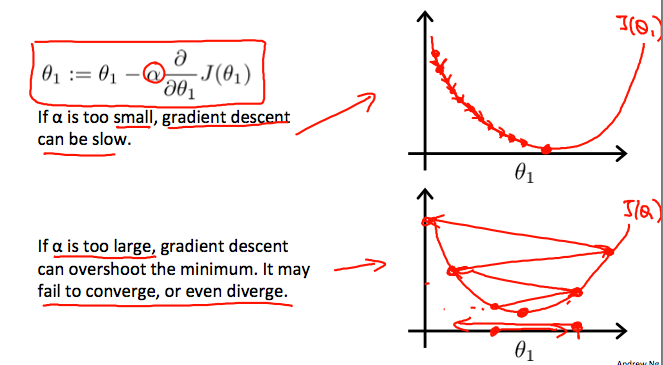
\includegraphics[width=1\textwidth]{img/UJpiD6GWEeai9RKvXdDYag_3c3ad6625a2a4ec8456f421a2f4daf2e_Screenshot-2016-11-03-00.05.27.png}
    \caption{}\label{GradientDescent3}
\end{figure}
Un'idea sarebbe quella di cambiare il valore di $\alpha$ al variare della discesa, in modo da evitare problematiche. Fortunatamente esiste un'intuizione che ci permette di far rimanere tale valore \textbf{costante} per tutto l'algoritmo. Ricordiamo infatti che il valore della derivata \textbf{diminuisce} a ogni passo. Questo poiché $\frac{d}{d\theta_1} J(\theta_1) \to 0$. Al minimo infatti avremo: 
\[\theta_1:=\theta_1-\alpha * 0\]
Quindi di step da effettuare diverranno sempre più piccoli.
\begin{figure}[h!]
    \centering
    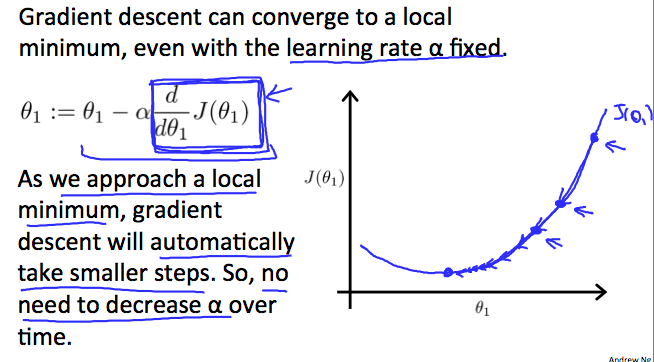
\includegraphics[width=1\textwidth]{img/RDcJ-KGXEeaVChLw2Vaaug_cb782d34d272321e88f202940c36afe9_Screenshot-2016-11-03-00.06.00.png}
    \caption{}\label{GradientDescent4}
\end{figure}
\subsection{Discesa del Gradiente per La Regressione Lineare}
\begin{align} \text{repeat until convergence: } \lbrace & \newline \theta_0 := & \theta_0 - \alpha \frac{1}{m} \sum\limits_{i=1}^{m}(h_\theta(x_{i}) - y_{i}) \newline \theta_1 := & \theta_1 - \alpha \frac{1}{m} \sum\limits_{i=1}^{m}\left((h_\theta(x_{i}) - y_{i}) x_{i}\right) \newline \rbrace& \end{align}
TODO
\section{Regressione Logistica}
Nei problemi di classificazione binaria o multiclasse, ovvero quei casi in cui la \textbf{funzione target} di un dataset fornisce valori appartenenti a un insieme binario o a un insieme più ampio, è sconsigliato sfruttare un'ipotesi lineare per approssimare l'andamento del dataset. Il motivo è che la funzione target è una funzione che assume solo valori discreti in un determinato intervallo e, sebbene si possa ipotizzare di approssimare il tutto con un valore soglia, un'ipotesi lineare può assumere valori \textbf{continui} ipoteticamente per tutti i valori reali. Concentrandoci sui problemi di \textbf{classificazione binaria}, la risoluzione del problema avviene mediante l'utilizzo di ipotesi logistiche (\textbf{regressione logistica}). 
\subsection{Classificazione e Rappresentazione}
La regressione logistica è espressa per mezzo della funzione logistica (chiamata anche \textbf{Sigmoide}):
$$ g(z) = \dfrac{1}{1 + e^{-z}} $$ 
\begin{center}
    \begin{tikzpicture}
    \begin{axis}[
        height = 7.3cm,
        width = 11cm,
        title = {sigmoid function},
        axis on top = true,
        axis x line = bottom,
        axis y line = left,
        x axis line style = -,
        y axis line style = -,
        tick align = outside,
        every tick/.append style = {
            black,
            thin
        },
%       grid = major,
        ymin = 0,
        ymax = 1,
        xlabel = $z$
    ]
        \addplot[
            blue,
            domain = -5:5,
            samples = 100
        ]
            {1/(1+exp(-x))};
    \end{axis}
\end{tikzpicture}
\end{center}
La funzione logistica possiede una peculiarità: \textbf{può assumere valori continui solo in $[0,1]$}. \\ Per necessità esprimiamo il tutto usando le seguenti uguaglianze:
\begin{align*}& h_\theta (x) = g ( \theta^T x ) \\& z = \theta^T x \\& g(z) = \dfrac{1}{1 + e^{-z}}\end{align*}
Interpretiamo $h_\theta (x)$ come \textbf{la probabilità che $y(x)=1$ su input $x$}:
\begin{align*}& h_\theta(x) = P(y=1 | x ; \theta) = 1 - P(y=0 | x ; \theta) \\& P(y = 0 | x;\theta) + P(y = 1 | x ; \theta) = 1\end{align*}
Per ottenere, come da ipotesi, una classificazione discreta di 0 o 1, sfruttiamo un valore soglia tale per cui:
\begin{align*}& h_\theta(x) \geq 0.5 \rightarrow y = 1 \\& h_\theta(x) < 0.5 \rightarrow y = 0 \\\end{align*}
Il modo in cui si comporta quindi la funzione logistica è il seguente:
\begin{align*}& g(z) \geq 0.5 \\& when \; z \geq 0\end{align*}
Ora bisogna solo capire \textbf{quando la funzione logistica assume determinanti valori}, in particolare affermiamo:
\begin{align*}& h_\theta(x) = g(\theta^T x) \geq 0.5 \\& when \; \theta^T x \geq 0\end{align*}
Secondo queste ipotesi allora giungiamo alla conclusione che in valore dell'input fornisce un valore d'output secondo tale approssimazione:
\begin{align*}& \theta^T x \geq 0 \Rightarrow y = 1 \\& \theta^T x < 0 \Rightarrow y = 0 \newline\end{align*}
\subsubsection{Decision Boundary}
Il confine decisionale (\textbf{Decision Boundary}) è una linea che separa l'area del grafico per cui $y=0$ da quella per cui $y=1$. Essa è una \textbf{particolarità} della funzione (in relazione all'input $x$ e ai valori fissati $\theta_i$) e \textbf{non} riguarda il dataset.
\begin{definizione}[]Decision Boundary from Wikipedia]
  In a statistical-classification problem with two classes, a decision boundary \cite{ConfineDecisionale} or decision surface is a hypersurface that partitions the underlying vector space into two sets, one for each class. The classifier will classify all the points on one side of the decision boundary as belonging to one class and all those on the other side as belonging to the other class. A decision boundary is the region of a problem space in which the output label of a classifier is ambiguous.If the decision surface is a hyperplane, then the classification problem is linear, and the classes are linearly separable.Decision boundaries are not always clear cut. That is, the transition from one class in the feature space to another is not discontinuous, but gradual. This effect is common in fuzzy logic based classification algorithms, where membership in one class or another is ambiguous
\end{definizione}
\begin{nota}
In the case of backpropagation based artificial neural networks or perceptrons, the type of decision boundary that the network can learn is determined by the number of hidden layers the network has. If it has no hidden layers, then it can only learn linear problems. If it has one hidden layer, then it can learn any continuous function on compact subsets of Rn as shown by the Universal approximation theorem, thus it can have an arbitrary decision boundary. In particular, support vector machines find a hyperplane that separates the feature space into two classes with the maximum margin. If the problem is not originally linearly separable, the kernel trick can be used to turn it into a linearly separable one, by increasing the number of dimensions. Thus a general hypersurface in a small dimension space is turned into a hyperplane in a space with much larger dimensions. Neural networks try to learn the decision boundary which minimizes the empirical error, while support vector machines try to learn the decision boundary which maximizes the empirical margin between the decision boundary and data points. 
\end{nota}
\begin{esempio}
  \begin{align*}& \theta = \begin{bmatrix}5 \\ -1 \\ 0\end{bmatrix} \\ & y = 1 \; if \; 5 + (-1) x_1 + 0 x_2 \geq 0 \\ & 5 - x_1 \geq 0 \\ & - x_1 \geq -5 \\& x_1 \leq 5 \\ \end{align*}
    \begin{figure}[h!]
        \centering
        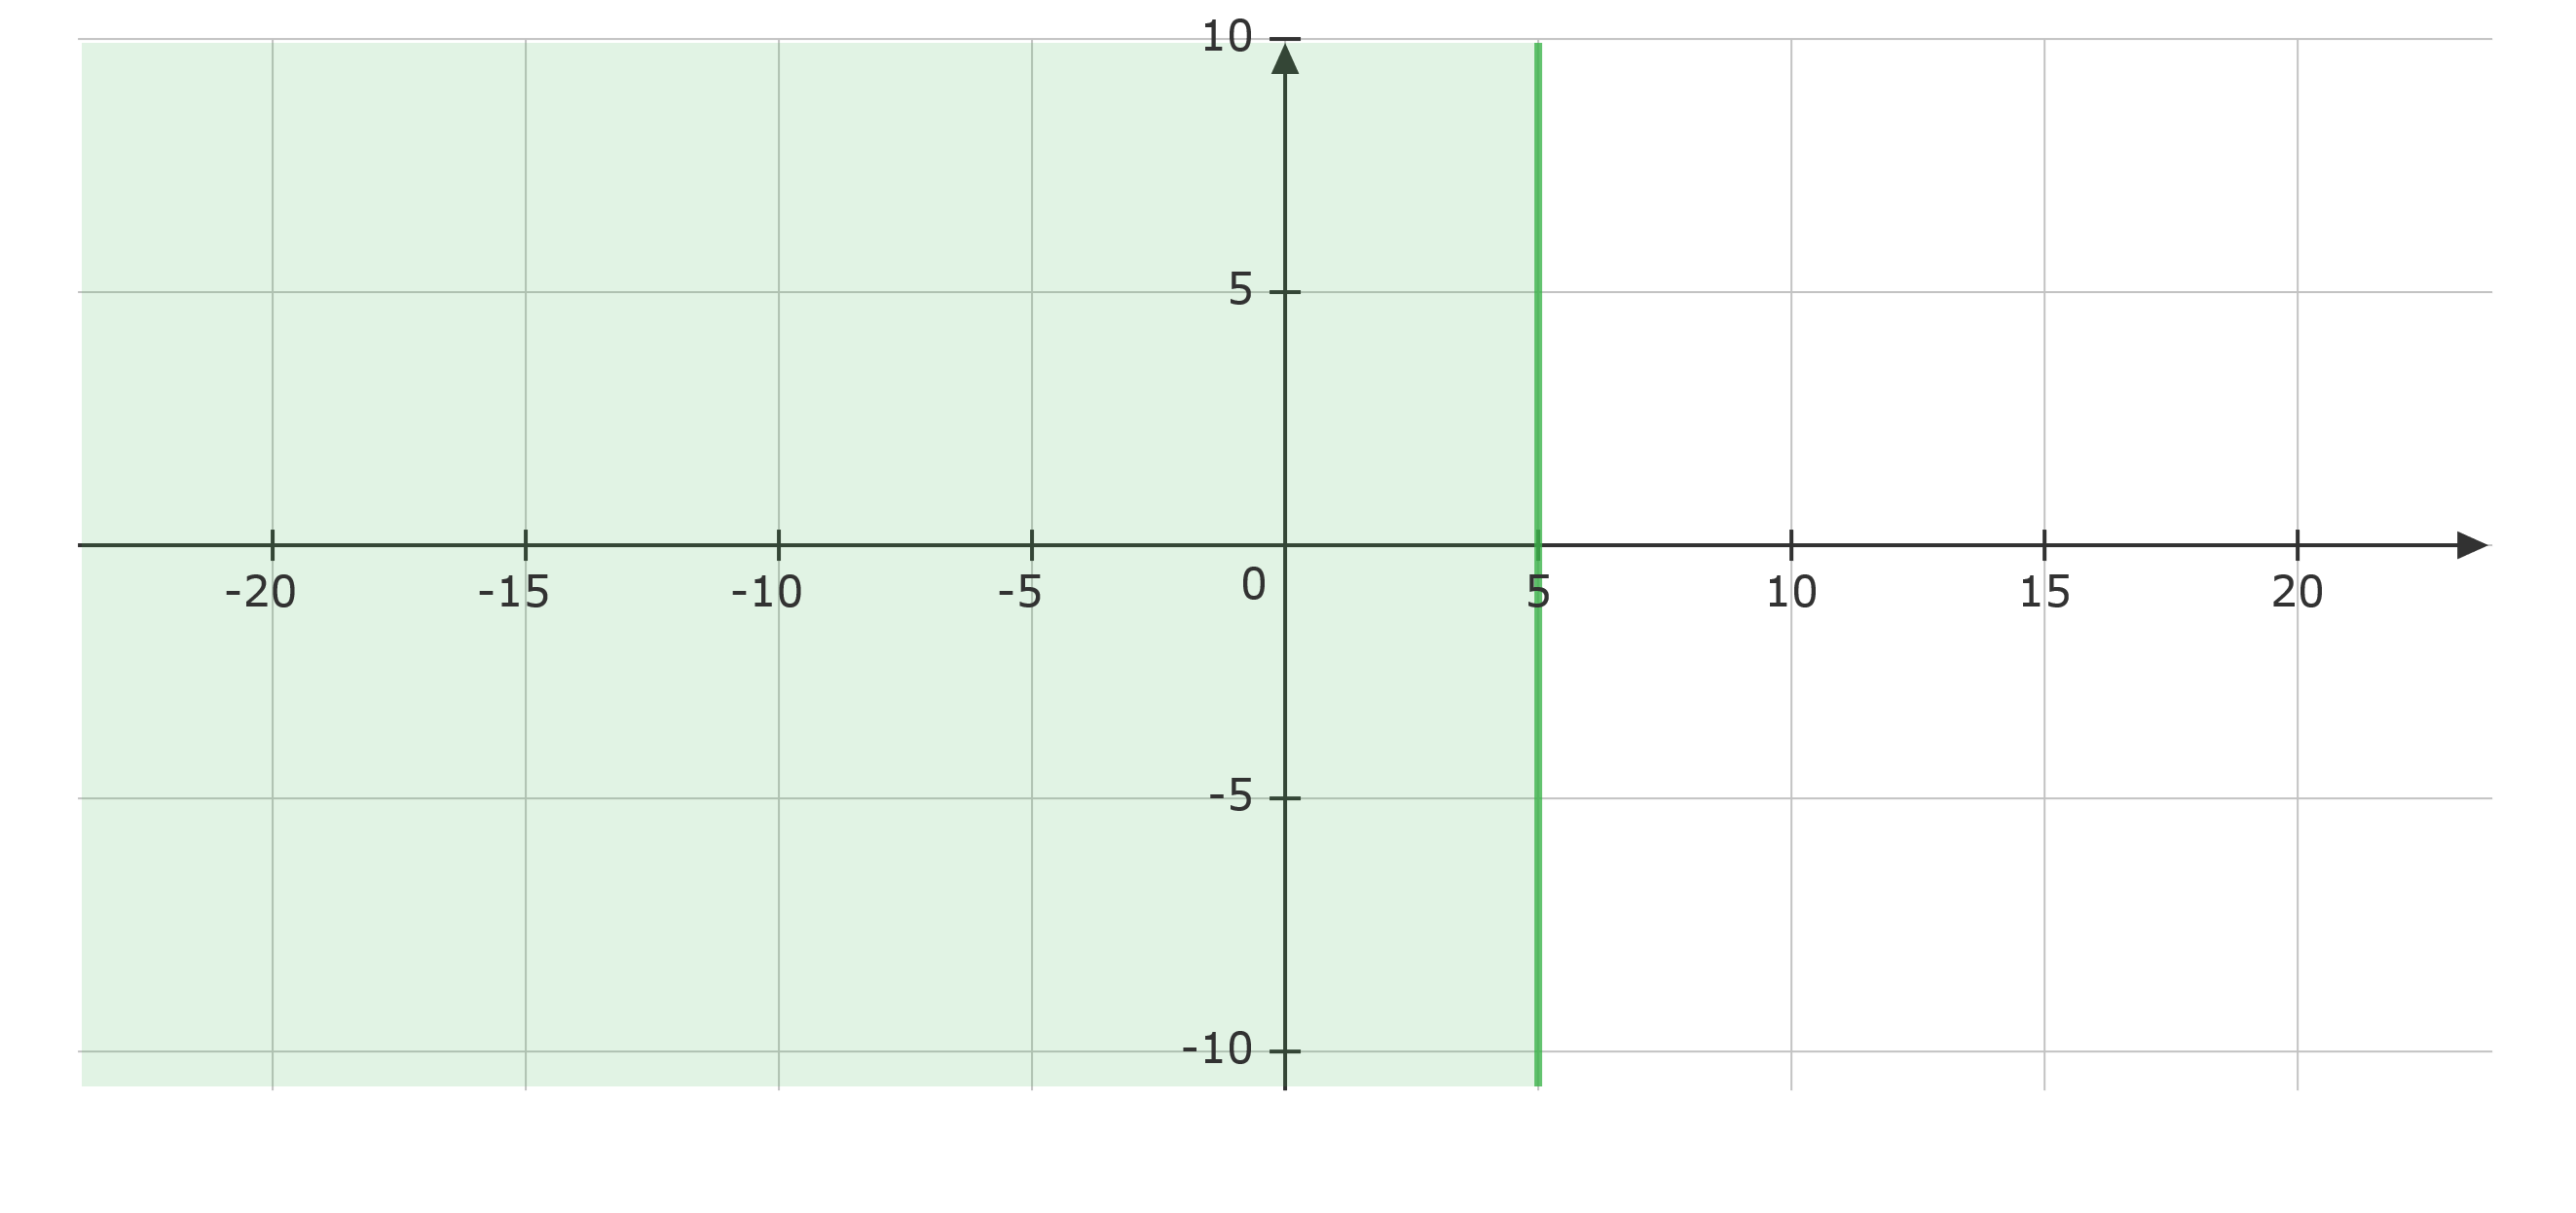
\includegraphics[width=1\textwidth]{img/diagram-1.png}
    \end{figure}
\end{esempio}
Ricordiamo che la funzione logistica è una funzione che non prevede, forzatamente, un input $\theta^T x$ lineare. 
\subsection{Modello di regressione logistica}
Ora i lettori si domanderanno: \textit{"Mario, ma come possiamo quindi decidere il valore da dare all'input?"}. L'input $x$ viene fornito solitamente da un dataset, sebbene la funzione logistica sia una funzione in $x$ dato $\theta_i$ fissati. Quindi la vera domanda è:\textit{ "Come facciamo a scegliere i valori di $\theta$?"}. Per far ciò introduciamo la \textbf{funzione di costo} della nostra funzione logistica:
\begin{align*}& J(\theta) = \dfrac{1}{m} \sum_{i=1}^m \mathrm{Cost}(h_\theta(x^{(i)}),y^{(i)}) \\ & \mathrm{Cost}(h_\theta(x),y) = -\log(h_\theta(x)) \; & \text{if y = 1} \\ & \mathrm{Cost}(h_\theta(x),y) = -\log(1-h_\theta(x)) \; & \text{if y = 0}\end{align*}
Che in maniera compatta si potrebbe scrivere come:
\[J(\theta) = - \frac{1}{m} \displaystyle \sum_{i=1}^m [y^{(i)}\log (h_\theta (x^{(i)})) + (1 - y^{(i)})\log (1 - h_\theta(x^{(i)}))]\]
\[\mathrm{Cost}(h_\theta(x),y) = - y \; \log(h_\theta(x)) - (1 - y) \log(1 - h_\theta(x))\]
Sfortunatamente tale funzione di costo differisce da quella della regressione lineare, poiché essa (prendendo in considerazione l'ipotesi logistica, quindi basata su una funzione sigmoide) non sarebbe una funzione convessa e quindi sarebbe complicato applicare la \textbf{discesa del gradiente} per trovarne il minimo.\\
\begin{figure}[!htb]
   \begin{minipage}{0.48\textwidth}
     \centering
     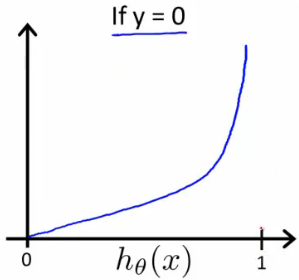
\includegraphics[width=.7\linewidth]{img/Ut7vvXnxEead-BJkoDOYOw_f719f2858d78dd66d80c5ec0d8e6b3fa_Logistic_regression_cost_function_negative_class.png}
     \caption{Funzione di costo per $y(x) = 0$}\label{Fig:y0}
   \end{minipage}\hfill
   \begin{minipage}{0.48\textwidth}
     \centering
     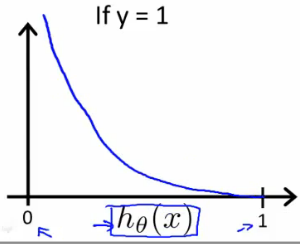
\includegraphics[width=.7\linewidth]{img/Q9sX8nnxEeamDApmnD43Fw_1cb67ecfac77b134606532f5caf98ee4_Logistic_regression_cost_function_positive_class.png}
     \caption{Funzione di costo per $y(x) = 1$}\label{Fig:y1}
   \end{minipage}
\end{figure}
Dalle figure \ref{Fig:y0} e \ref{Fig:y1} si noti che la funzione di costo penalizza un determinato algoritmo nel caso in cui l'osservazione sia differente rispetto all'interpretazione dell'ipotesi, ovvero:
\begin{align*}& \mathrm{Cost}(h_\theta(x),y) = 0 \text{ if } h_\theta(x) = y \\ & \mathrm{Cost}(h_\theta(x),y) \rightarrow \infty \text{ if } y = 0 \; \mathrm{and} \; h_\theta(x) \rightarrow 1 \\ & \mathrm{Cost}(h_\theta(x),y) \rightarrow \infty \text{ if } y = 1 \; \mathrm{and} \; h_\theta(x) \rightarrow 0 \\ \end{align*}
Per trovare i parametri $\theta$ sfruttiamo la \textbf{discesa del gradiente per $J(\theta)$}:
\begin{align*}& Repeat \; \lbrace \\ & \; \theta_j := \theta_j - \alpha \dfrac{\partial}{\partial \theta_j}J(\theta) \\ & \rbrace\end{align*}
Svolgendo la derivata parziale avremo un valore \textbf{simile} a quello della regressione lineare, con un'unica differenza: l'ipotesi $h_\theta(x)$ è una funzione logistica/sigmoide in questo caso.
\begin{align*} & Repeat \; \lbrace \\ & \; \theta_j := \theta_j - \frac{\alpha}{m} \sum_{i=1}^m (h_\theta(x^{(i)}) - y^{(i)}) x_j^{(i)} \\ & \rbrace \end{align*}
L'algoritmo per la discesa del gradiente riporta il valore minimo di $J$ in base a un determinato valore di $\theta$.
\section{Bias Induttivo}
Nelle future trattazioni ricorrerà spesso la nozione di \textbf{bias induttivo}. Se ne vuole perciò fornire un'introduzione a priori per favorire l'apprendimento degli esempi che seguiranno nel corso della trattazione.
\begin{definizione}[\textbf{Bias Induttivo}]
  From \href{https://it.wikipedia.org/wiki/Bias_induttivo}{Wikipedia}: Nell'apprendimento automatico, il bias induttivo di un algoritmo è l'insieme di assunzioni che il classificatore usa per predire l'output dati gli input che esso non ha ancora incontrato (Mitchell, 1980).

L'apprendimento automatico mira a costruire algoritmi che siano in grado di apprendere una certa \textbf{funzione obiettivo}. A tale scopo, si fornisce all'algoritmo di apprendimento un insieme di addestramento, che contiene esempi della relazione sottesa tra valori d'ingresso e di uscita della funzione obiettivo. Il classificatore deve quindi approssimare la funzione obiettivo a partire da tali esempi. Il tipo di assunzioni che il classificatore effettua sulla natura della funzione obiettivo prende il nome di bias induttivo (Mitchell, 1980; desJardins and Gordon, 1995).

Un classico esempio di bias induttivo è il rasoio di Occam (che verrà nominato spesso nel corso della trattazione di questo libro). Tale principio assume che l'ipotesi più semplice consistente con l'insieme di addestramento sia da preferire. 
\end{definizione}
Più formalmente:
\begin{definizione} 
  Il \textbf{bias induttivo} di $L$ è un insieme
  minimale di asserzioni $B$ tale 
  che, per ogni concetto target $c$ e $D_c$ corrispondente si ha che:
  \[[B\land D_c\land x_i]\,\vdash\, L(x_i, D_c),\,\,\forall x_i\in X\]
  con $\vdash$ che rappresenta l'implicazione logica
\end{definizione}
\section{Ripasso di Algebra Lineare}
									      			      		\begin{shaded}
									      			      			\textbf{Ripasso di algebra lineare}\\
									      			      			Per praticità ripasseremo i concetti fondamentali facendo riferimento a
									      			      			$\mathbb{R}^2$, formato quindi da elementi, dette coordinate, che sono coppie
									      			      			ordinate $(x_1, x_2)$ (rappresentabili con un punto nel piano o con un segmento
									      			      			orientato con partenza nell'origine e destinazione nelle coordinate del punto
									      			      			nel piano).\\
									      			      			Ricordiamo le operazioni fondamentali, dati $R$ pari a $(x_1, x_2)$ e $Q$ pari
									      			      			a $(x_3, x_4)$ 
									      			      			\begin{itemize}
									      			      				\item addizione: $P+Q=(x_1+x_3, x_2+x_4)$
									      			      				\item prodotto per uno scalare $\alpha\in\mathbb{R}$: $\alpha\cdot
									      			      				      R=(\alpha\cdot x_1,\alpha\cdot x_2)$
									      			      				\item prodotto scalare tra vettori: $\langle P, Q\rangle\equiv P\cdot Q^T =
									      			      				      \sum_{i=1}^n r_i\cdot q_i$ 
									      			      				      (dove $r_i$ e $q_i$ sono rispettivamente gli elementi di $R$ e $Q$
									      			      				      all'indice $i$)
									      			      			\end{itemize}
									      			      			Ricordiamo la \textit{norma} di un vettore $X$:
									      			      			\[\norm{X}=\equiv\sqrt{X\cdot X^T}=\sqrt{\sum_{i=1}^n x_i\cdot
									      			      					x_i}=\sqrt{\langle X, X\rangle}\] 
									      			      				Con $X=0$ indichiamo il \textit{vettore nullo} (che ha anche norma nulla).\\
									      			      				Definiamo il \textit{versore} (\textit{vettore unitario}) come:
									      			      				\[\frac{X}{\norm{X}},\,\,\, X\neq 0\]
									      			      				In $\mathbb{R}^2$ l'angolo $\theta$ sotteso tra due vettori $X$ e $Y$ è:
									      			      				\[\cos\theta=\frac{\langle X, Y\rangle}{\norm{X}\cdot \norm{Y}}\]
									      			      				La proiezione di un vettore $X$ sul vettore $Y$ è:
									      			      				\[X_Y=\norm{X}\cdot \cos\theta\]
									      			      				Si hanno quindi tre casi:
									      			      				\begin{enumerate}
									      			      					\item $\theta < 90 \iff \langle X, Y\rangle >0$
									      			      					\item $\theta > 90 \iff \langle X, Y\rangle <0$
									      			      					\item $\theta = 90 \iff \langle X, Y\rangle =0$
									      			      				\end{enumerate}
									      			      				(quindi disegnando una retta sul piano tutti i punti sopra di essa
									      			      				apparterranno a una certa classe e quelli sotto a un'altra).\\
									      			      				Posso definire una retta $r$ che passa per l'origine in  $\mathbb{R}^2$
									      			      				assegnando un vettore $W=(w_1, w_2)$ ad essa ortogonale, infatti tutti i punti,
									      			      				ovvero vettori, $X=(x_1, x_2)$ sulla retta sono ortogonali a $W$:
									      			      				\[\langle W, X\rangle=w_1\cdot x_1+w_2\cdot x_2=0 \]
									      			      				Quindi la retta (ovvero l'iperpiano) mi separa due semispazi, a seconda che
									      			      				$\langle X, W\rangle$ sia strettamente positivo o strettamente negativo.\\
									      			      				Generalizzando ora a $n$ dimensioni ho che, dato l'iperpiano $h$ (di
									      			      				dimensione $n-1$):
									      			      				\begin{itemize}
									      			      					\item se $h$ passa dall'origine allora si ha l'equazione $\langle X, Y\rangle
									      			      					      =0$
									      			      					\item se non passa per l'origine $\langle X, Y\rangle +b=0$ 
									      			      					          
									      			      				\end{itemize}
									      			      				I vettori in un iperpiano si proiettano tutti nello stesso modo e i punti ad
									      			      				un lato e all'altro dell'iperpiano sono distinti dal fatto che $\langle
									      			      				X, Y\rangle +b$ sia strettamente positiva o strettamente negativa
									      			      				\end{shaded}
